\let\negmedspace\undefined
\let\negthickspace\undefined
\documentclass[journal,12pt,onecolumn]{IEEEtran}
\usepackage{cite}
\usepackage{amsmath,amssymb,amsfonts,amsthm}
\usepackage{algorithmic}
\usepackage{graphicx}
\graphicspath{{./figs/}}
\usepackage{textcomp}
\usepackage{xcolor}
\usepackage{txfonts}
\usepackage{listings}
\usepackage{enumitem}
\usepackage{mathtools}
\usepackage{gensymb}
\usepackage{comment}
\usepackage{caption}
\usepackage[breaklinks=true]{hyperref}
\usepackage{tkz-euclide} 
\usepackage{listings}
\usepackage{gvv}                                        
%\def\inputGnumericTable{}                                 
\usepackage[latin1]{inputenc}     
\usepackage{xparse}
\usepackage{color}                                            
\usepackage{array}
\usepackage{longtable}                                       
\usepackage{calc}                                             
\usepackage{multirow}
\usepackage{multicol}
\usepackage{hhline}                                           
\usepackage{ifthen}                                           
\usepackage{lscape}
\usepackage{tabularx}
\usepackage{array}
\usepackage{float}
\newtheorem{theorem}{Theorem}[section]
\newtheorem{problem}{Problem}
\newtheorem{proposition}{Proposition}[section]
\newtheorem{lemma}{Lemma}[section]
\newtheorem{corollary}[theorem]{Corollary}
\newtheorem{example}{Example}[section]
\newtheorem{definition}[problem]{Definition}
\newcommand{\BEQA}{\begin{eqnarray}}
\newcommand{\EEQA}{\end{eqnarray}}
\newcommand{\define}{\stackrel{\triangle}{=}}
\theoremstyle{remark}
\newtheorem{rem}{Remark}

\begin{document}

\title{5.5.8}
\author{ee25btech11056 - Suraj.N}
\maketitle
\renewcommand{\thefigure}{\theenumi}
\renewcommand{\thetable}{\theenumi}

\begin{document}

\textbf{Question :}  If 
\[
\vec{A} = \myvec{1 & 1 & 1 \\ 0 & 1 & 3 \\ 1 & -2 & 1}
\]
find $\vec{A}^{-1}$. Hence, solve the system of equations
\[
x+y+z=6,\quad y+3z=11,\quad x-2y+z=0.
\]

\textbf{Solution :}

\begin{table}[h!]
  \centering
  \begin{tabular}{|c|c|}
\hline
\textbf{Name} & \textbf{Value} \\ \hline
$\vec{A}$ & $\myvec{2 & 1 \\0 & 3}$ \\ \hline
\end{tabular}

  \caption*{Table : Matrices}
  \label{5.5.8}
\end{table}

Forming the augmented matrix,

\begin{align}
  \myaugvec{3}{1 & 1 & 1 & 1 & 0 & 0\\0 & 1 & 3 & 0 & 1 & 0\\1 & -2 & 1 & 0 & 0 & 1 }
\end{align}

Applying elementary row operations to find the inverse,

\begin{align}
\myaugvec{3}{1 & 1 & 1 & 1 & 0 & 0\\0 & 1 & 3 & 0 & 1 & 0\\1 & -2 & 1 & 0 & 0 & 1 }
\xleftrightarrow{\;R_3 \to R_3 - R_1}
\myaugvec{3}{1 & 1 & 1 & 1 & 0 & 0\\0 & 1 & 3 & 0 & 1 & 0\\0 & -3 & 0 & -1 & 0 & 1 }
\xleftrightarrow{\;R_3 \to R_3 + 3R_2}
\myaugvec{3}{1 & 1 & 1 & 1 & 0 & 0\\0 & 1 & 3 & 0 & 1 & 0\\0 & 0 & 9 & -1 & 3 & 1 }
\end{align}

\begin{align}
\myaugvec{3}{1 & 1 & 1 & 1 & 0 & 0\\0 & 1 & 3 & 0 & 1 & 0\\0 & 0 & 9 & -1 & 3 & 1 }
\xleftrightarrow{\;R_3 \to \tfrac{R_3}{9}}
\myaugvec{3}{1 & 1 & 1 & 1 & 0 & 0\\0 & 1 & 3 & 0 & 1 & 0\\0 & 0 & 1 & -\tfrac{1}{9} & \tfrac{1}{3} & \tfrac{1}{9} }
\xleftrightarrow[\;R_1 \to R_1 - R_3\;]{\;R_2 \to R_2 - 3R_3}
\myaugvec{3}{1 & 1 & 0 & \tfrac{10}{9} & -\tfrac{1}{3} & -\tfrac{1}{9}\\0 & 1 & 0 & \tfrac{1}{3} & 0 & -\tfrac{1}{3}\\0 & 0 & 1 & -\tfrac{1}{9} & \tfrac{1}{3} & \tfrac{1}{9} }
\end{align}

\begin{align}
\myaugvec{3}{1 & 1 & 0 & \tfrac{10}{9} & -\tfrac{1}{3} & -\tfrac{1}{9}\\0 & 1 & 0 & \tfrac{1}{3} & 0 & -\tfrac{1}{3}\\0 & 0 & 1 & -\tfrac{1}{9} & \tfrac{1}{3} & \tfrac{1}{9} }
\xleftrightarrow{\;R_1 \to R_1 - R_2}
\myaugvec{3}{1 & 0 & 0 & \tfrac{7}{9} & -\tfrac{1}{3} & \tfrac{2}{9}\\0 & 1 & 0 & \tfrac{1}{3} & 0 & -\tfrac{1}{3}\\0 & 0 & 1 & -\tfrac{1}{9} & \tfrac{1}{3} & \tfrac{1}{9} }
\end{align}

\pagebreak

The right side part of the augmented matrix is $\vec{A}^{-1}$

\begin{align}
  \vec{A}^{-1} &= \myvec{\tfrac{7}{9} & -\tfrac{1}{3} & \tfrac{2}{9}\\\tfrac{1}{3} & 0 & -\tfrac{1}{3}\\-\tfrac{1}{9} & \tfrac{1}{3} & \tfrac{1}{9}}
\end{align}

The solution for the system of equations is :

\begin{align}
  \vec{A}\vec{x} &= \vec{b}\\
  \vec{x} &= \vec{A}^{-1}\vec{b}\\
  \myvec{x\\y\\z} &= \myvec{\tfrac{7}{9} & -\tfrac{1}{3} & \tfrac{2}{9}\\\tfrac{1}{3} & 0 & -\tfrac{1}{3}\\-\tfrac{1}{9} & \tfrac{1}{3} & \tfrac{1}{9}}\myvec{6\\11\\0}\\
  \myvec{x\\y\\z} &= \myvec{1\\2\\3}
\end{align}

Therefore the solution is :

\begin{align}
\myvec{x\\y\\z} &= \myvec{1\\2\\3}
\end{align}

\pagebreak

\begin{figure}[h!]
  \centering
  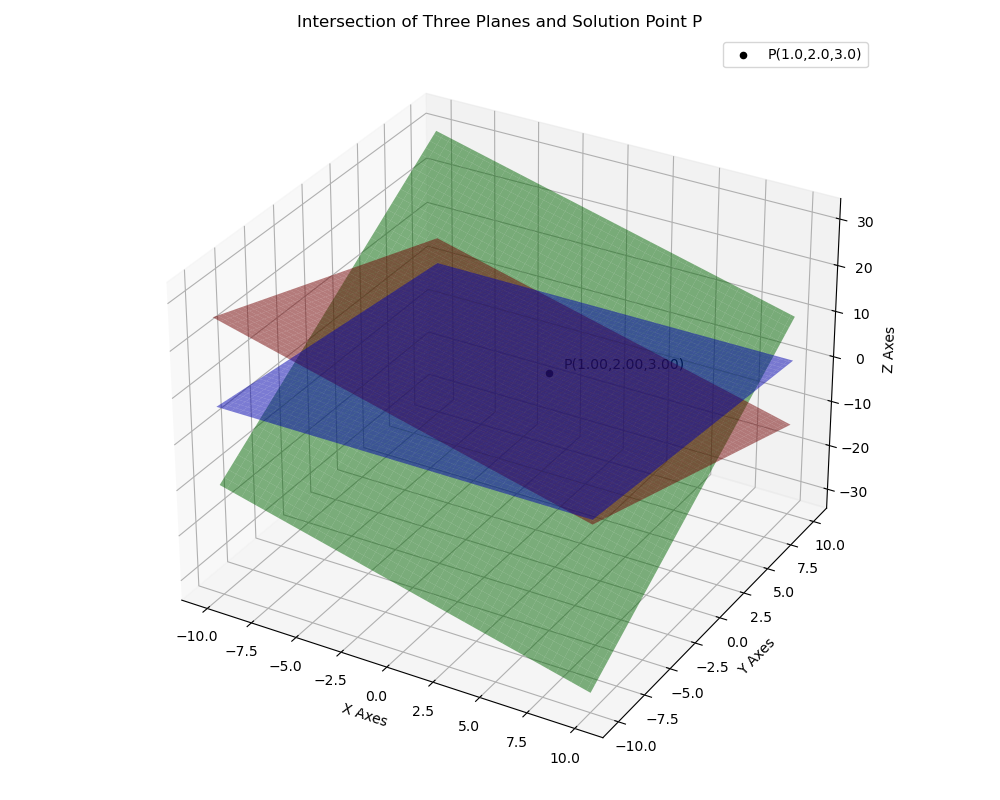
\includegraphics[width=0.7\columnwidth]{figs/solution.png} 
   \caption*{Fig : Planes}
  \label{Fig1}
\end{figure}


\end{document}
